\documentclass[journal=ascecg,manuscript=article]{achemso}

\usepackage[version=4]{mhchem} % Formula subscripts using \ce{}
\usepackage{import}
\usepackage{multirow}
\usepackage{adjustbox}
\usepackage{subcaption}
\usepackage{amsmath}
\usepackage{xcolor}
\usepackage{ulem}
\usepackage{amssymb}
\usepackage{array}
\usepackage[utf8]{inputenc}
\usepackage[T1]{fontenc}
%\usepackage{mathptmx}
\usepackage{etoolbox}
%\usepackage[version=4]{mhchem}
\usepackage{float}
\usepackage{tabularx}
%%\listfiles

\newcommand*\mycommand[1]{\texttt{\emph{#1}}}

\author{Felipe Mourão Coelho}
\affiliation{Universidade Estadual de Campinas (UNICAMP), Faculdade de Engenharia Química, Campinas-SP, 13083-852, Brazil}

\author{Luís Fernando Mercier Franco}
\affiliation{Universidade Estadual de Campinas (UNICAMP), Faculdade de Engenharia Química, Campinas-SP, 13083-852, Brazil}
 \email{lmfranco@unicamp.br}

 \author{Abbas Firoozabadi}
\affiliation{Rice University, Houston-TX, 77005, USA}
\email{abbas.firoozabadi@rice.edu}



\title[An \textsf{achemso} demo]
  {Phase Equilibria of \ce{CO2}-Water and \ce{CO2}-Brine at High Temperature: from Monte Carlo Simulations to Equation of State} 



\keywords{Geothermal Energy, Phase Equilibria, \ce{CO2}, Gibbs Ensenble Monte Carlo, Association, CPA, Electrolytes}

\begin{document}

\begin{tocentry}
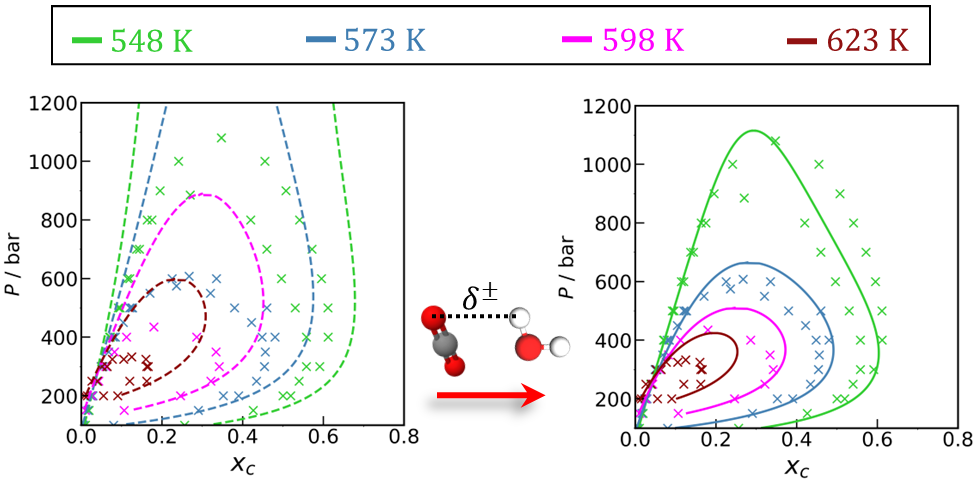
\includegraphics{Figures/TOC.png}
\end{tocentry}

\begin{abstract}
Accurate modeling of \ce{CO2} partitioning in the \ce{CO2}-water and \ce{CO2}-brine systems and density of equilibrium phases over a wide pressure range at temperatures from  50 to 500 °C are of high interest in many subsurface processes. The conditions relate to geothermal formations and \ce{CO2} sequestration in saline aquifers. Geothermal is a renewable energy resource and may provide an alternative to fossil fuel energy. \ce{CO2} sequestration is considered as the key to mitigate \ce{CO2} release to the atmosphere. Current modeling is primarily based on various correlations and equations of state, such as the cubic-plus-association (CPA) and the electrolyte CPA (eCPA). When partitioning and phase volumetric properties are computed based on CPA and eCPA, deficiencies and inaccuracies emerge, especially in the range of applications for geothermal formations (higher temperatures). The use of correlations has limitations. We parametrize a new set of CPA and eCPA equations of state accounting for the \ce{CO2}-\ce{H2O} cross-association. The \ce{CO2}-water phase diagrams are reproduced for temperatures over 600 K, and the mutual solubility is described at temperatures as low as 300 K. The eCPA predicts the solubility of \ce{CO2} in NaCl brine up to about 700 K and 6 m of salinity. The density of \ce{CO2} in aqueous mixtures is reproduced accurately  (within 1\%). eCPA can predict the aqueous phase density increase and decrease from \ce{CO2} dissolution depending on temperature and salinity. From Monte Carlo simulations, the SPCE-EPM2 force field with optimized unlike parameters captures the high-temperature phase diagram (to about 600 K) without polarization corrections. Association structural parameters from both molecular simulation and equation of states are in agreement. We show that \ce{CO2}-\ce{H2O} cross-association is significant from a molecular perspective. In this work, the knowledge of the thermodynamics of  \ce{CO2}-water and \ce{CO2}-brine mixtures is expanded by providing a model for geothermal and \ce{CO2} sequestration conditions.    
\end{abstract} 



    \import{}{1Intro.tex}
    \import{}{2Method.tex}
    \import{}{3Results.tex}
    \import{}{4Conc.tex}
    



\begin{acknowledgement}
The authors thanks the São Paulo Research Foundation (FAPESP) for the project funding (grants: \#2018/02713-8, \#2020/13300-6, and \#2021/13068-9), the ``Centro Nacional de Processamento de Alto Desempenho em São Paulo'' (CENAPAD-SP) and the John David Rogers Computing Center (CCJDR) at the Institute of Physics ``Gleb Wataghin'' of the University of Campinas for providing computational resources,
the Coordenação de Aperfeiçoamento de Pessoal de Nível Superior (CAPES) Brasil for Financial Support, and the Conselho Nacional de Desenvolvimento Científico e Tecnológico (CNPq) Brasil.
\end{acknowledgement}


\begin{suppinfo}
The Supplementary Material contains the derivation of the compressibility factor, fugacity coefficient and relative permittivity; pure parameters for the equation of state and molecular simulations;  CPA and eCPA phase equilibria at lower temperatures; comparison between our CPA and eCPA with others from the Literature; density of the aqueous phase below \ce{CO2} saturation with and without salt; comparison between the performance of various force fields in the phase equilibria; density of phases in equilibrium from CPA/eCPA and GEMC; composition of the \ce{CO2}-rich phase in the \ce{CO2}-brine mixture; scheme of radial distribution functions; influence of  unlike parameters on association in MD simulations.
\end{suppinfo}

\newpage
\bibliography{5REF}

\end{document}
